\documentclass[12pt]{article}
\usepackage{kotex}
\usepackage{amsmath}
\usepackage{amsfonts}
\usepackage{amssymb}
\usepackage{amsthm}
\usepackage{mathtools}
\usepackage{extarrows}
\usepackage{amscd}
\usepackage{titlesec}
\usepackage{chngcntr}
\usepackage{tikz-cd} 
\usepackage{fancyhdr}
\usepackage[utf8]{inputenc}
\usepackage[a4paper]{geometry}
\geometry{
	top = 20mm,
	bottom = 20mm,
	left = 20mm,
	right = 20mm
}

\usepackage{hyperref}
\hypersetup{
	colorlinks=true,
	linkcolor=black
}

\usepackage{enumitem}
\setlist[enumerate,1]{label={(\arabic*)}}

\setcounter{tocdepth}{2}
\setcounter{section}{0}

\counterwithin*{footnote}{section}
% \pagenumbering{gobble}
\renewcommand{\baselinestretch}{1.3}

\newcommand{\ds}{\displaystyle}
\newcommand{\abs}[1]{\left|#1\right|}
\newcommand{\paren}[1]{\left( #1 \right)}
\newcommand{\ceil}[1]{\left\lceil #1 \right\rceil}
\newcommand{\floor}[1]{\left\lfloor #1 \right\rfloor}
\renewcommand{\span}[1]{\left\langle #1 \right\rangle}
\newcommand{\norm}[1]{\left\lVert #1 \right\rVert}
\newcommand{\mf}[1]{\mathfrak{#1}}
\newcommand{\rmbf}[1]{\mathrm{\mathbf{#1}}}
\newcommand{\mc}[1]{\mathcal{#1}}
\newcommand{\bb}[1]{\mathbb{#1}}
\newcommand{\inv}{^{-1}}
\newcommand{\cross}{^\times}
\newcommand{\trans}{^{\mathrm{\mathbf{t}}}}
\newcommand{\adj}{\text{*}}
\newcommand{\ra}{\rightarrow}
\newcommand{\imp}{\implies}
\newcommand{\impb}{\impliedby}
\newcommand{\bs}{\setminus}
\newcommand{\N}{\mathbb{N}}
\newcommand{\Z}{\mathbb{Z}}
\newcommand{\Q}{\mathbb{Q}}
\newcommand{\R}{\mathbb{R}}
\newcommand{\C}{\mathbb{C}}
\newcommand{\F}{\mathbb{F}}
\DeclareMathOperator{\im}{im}
\DeclareMathOperator{\rk}{rk}
\DeclareMathOperator{\tr}{tr}
\DeclareMathOperator{\aut}{Aut}
\DeclareMathOperator{\diag}{diag}
\DeclareMathOperator{\ch}{char}
\DeclareMathOperator{\ann}{ann}
\DeclareMathOperator{\Ann}{Ann}
\newcommand{\nsub}{\mathrel{\unlhd}}
\newcommand{\pnsub}{\mathrel{\lhd}}
\newcommand{\mimp}{$\implies$}
\newcommand{\mimpb}{$\impliedby$}
\newcommand{\miff}{$\iff$}
\newcommand{\gop}{\text{곱}}
\newcommand{\sang}{\text{상}}
\newcommand{\tor}{_{\text{tor}}}

\renewcommand{\headrulewidth}{0.8pt}

\renewcommand{\contentsname}{목차}

\newcommand{\defn}[1]{\textbf{\sffamily Definition #1}}
\newcommand{\rmk}{\textbf{Remark}}
\newcommand{\ex}[1]{\textbf{\sffamily Example #1}}
\newcommand{\thm}[1]{\textbf{\sffamily Theorem #1}}
\newcommand{\pf}{\textit{Proof}}
\newcommand{\prop}[1]{\textbf{\sffamily Proposition #1}}
\newcommand{\prob}[1]{\textbf{\sffamily Exercise #1}}
\newcommand{\obs}[1]{\textbf{\sffamily Observation #1}}

\pagestyle{fancy}
\fancyhf{}
\lhead{\sffamily}
\rhead{\sffamily \thepage}

\title{\Large ~\\~\\~\\~\\학부 대수학 강의 II\\~\\~\\ \Huge \bfseries 대수학 \\~\\~\\~\\~\\}
\author{\itshape Sungchan Yi~\\~\\~\\}
\date{January, 2020}
\begin{document}
\maketitle
\pagebreak
\tableofcontents
\pagebreak

\section{Algebraic Structures I}
\subsection{Algebraic Structure}
\textbf{대수학}은 \textbf{algebraic structure}(\textbf{대수적 구조})를 공부하는 학문이다. 대수적 구조란 어떤 집합에 몇 개의 연산 구조가 주어진 것을 뜻한다. 우리는 \textbf{associative} binary operation 만을 생각한다.\footnote{모든 binary operation 은 associative 라고 가정한다.}\\
\\
\defn{1.1.1.} 이항연산 $\ast$ 를 갖는 집합 $G$ 가 다음 조건들
\begin{enumerate}
	\item[\sffamily (G1)] [모든 $g\in G$ 에 대하여 $g\ast e=e\ast g = g$] 인 원소 $e\in G$ 가 존재.
	\item[\sffamily (G2)] 각 $g \in G$ 에 대하여 [$g\ast \tilde{g} = \tilde{g}\ast g = e$ 인 원소 $\tilde{g}\in G$ 가 존재].
\end{enumerate}
을 만족하면 $(G, \ast)$ 를 \textbf{group}(\textbf{군}) 이라고 한다.\\

어떤 추가 조건들이 주어져 있는가에 따라 대수적 구조의 이름이 달라진다. 만약 위 정의에서 이항연산을 가진 집합 $G$ 가
\begin{enumerate}
	\item 아무런 추가 조건도 갖지 않으면 $G$ 를 \textbf{semigroup} 이라 한다.
	\item {\sffamily (G1)} 만을 만족하면, $G$ 를 \textbf{monoid} 라 한다.
	\item Group $G$ 가 $\abs{G}<\infty$ 도 만족하면, $G$ 를 \textbf{finite group} 이라 한다.
	\item Group $G$ 가 [$g\ast h = h\ast g$ for all $g, h\in G$] 도 만족하면 $G$ 를 \textbf{commutative group} (또는 \textbf{abelian group}) 이라 한다.
\end{enumerate}~
\\
\prob{1.1.3.} Consider $\N \cup \{0\}$ with addition. Associativity holds trivially, and $e = 0$. But there is no inverse for elements in $\N$.\\
\\
\defn{1.1.4.} $R$ 과 $X$ 가 집합일 때, 함수 $R\times X \ra X$ 를 $X$-위의 $R$-\textbf{상수곱} (\textbf{scalar multiplication}) 이라 한다. $a\in R$ 과 $x\in X$ 의 상수곱은 $a\cdot x = ax$ 로 표기한다. 또, $R$ 의 원소는 \textbf{scalar} 라고 부른다.\\
\\
\defn{1.1.7.} (\textbf{\sffamily Ring}) 집합 $R$ 이 \textbf{덧셈}과 \textbf{곱셈}이라는 이름의 두 개의 이항연산을 갖고 있을 때 다음 조건
\begin{enumerate}
	\item[\sffamily (R1)] $(a+b)c = ac+bc$, $a(b+c)=ab+ac$ \quad ($a, b, c\in R$) \quad (\textbf{분배법칙}(\textbf{distributive law}))
	\item[\sffamily (R2)] $(R, +)$ 는 abelian group
\end{enumerate}
을 만족하면, $(R, +, \gop)$ 을 \textbf{ring}(\textbf{환}) 이라 한다.\\
\\
\prob{1.1.8.} \textbf{Typical examples of ring}
\begin{enumerate}
	\item $(\Z, +,\gop)$
	\item $(\R, +,\gop)$
	\item $(\mf{M}_{n, n}(\R), +, \gop)$
	\item $(\R[t], +, \gop)$
\end{enumerate}
For all 4 examples, each set is an abelian group under addition, and the distributive law holds.\\

Alway remember: \textbf{우리가 아는 것은 행렬 뿐이다. 어떤 수학적 object 를 만나더라도 우리는 행렬(벡터공간)부터 생각한다.}\\
\\
\defn{1.1.10.} (\textbf{\sffamily $R$-module}) $R = (R, +, \gop)$ 이 ring 이고, 집합 $M$ 이 이항연산 \textbf{덧셈}과 $R$-\textbf{상수곱}을 갖고 있다고 하자.\footnote{$M$ 의 덧셈과 $R$ 의 덧셈은 분명히 구별해야 한다.} 다음 조건
\begin{enumerate}
	\item[\sffamily (M1)] $r(x+y) = rx + ry$ \quad ($r\in R,\;\; x, y, \in M$)
	\item[\sffamily (M2)] $(r+s)x = rx+sx$ \quad ($r, s\in R, \;\; x\in M$)
	\item[\sffamily (M3)] $r(sx) = (rs)x$ \quad ($r, s\in R, \;\; x\in M$)
	\item[\sffamily (M4)] $(M, +)$ 는 abelian group
\end{enumerate}
을 만족하면, $(M, +, \sang)$ 을 $R$-\textbf{module} ($R$-\textbf{가군}) 이라 한다.\\
\\
\prob{1.1.11.} \textbf{Typical examples of module}
\begin{enumerate}
	\item $x = (x_1, \dots, x_n), y = (y_1, \dots, y_n) \in \R^n$, $r, s\in \R$.
	\begin{enumerate}
		\item $r(x+y) = r(x_1+y_1, \dots, x_n+y_n) = (rx_1+ry_1, \dots, rx_n+ry_n) = rx+ry$
		\item $(r+s)x = (rx_1+sx_1, \dots, rx_n+sx_n) = rx + sx $
		\item $r(sx) = r(sx_1, \dots, sx_n) = (rsx_1, \dots, rsx_n) = (rs)x$
		\item Vector space $\R^n$ is an abelian group under addition.
	\end{enumerate}
	\item The proof is identical to (1).
\end{enumerate}~
\\
\prob{1.1.12.} $\R$-vector space was defined on a field ($\R$), while $R$-module is defined on a ring. A vector space over a field is a module over that field.\\
\\
\defn{1.1.13.} (\textbf{$R$-algebra}) $R=(R, +, \gop)$ 이 ring 이고, 집합 $\mc{A}$ 가 이항연산 \textbf{덧셈}과 \textbf{곱셈}, 그리고 $R$-\textbf{상수곱}을 갖고 있다고 하자. 다음 조건
\begin{enumerate}
	\item[\sffamily (A1)] $(\mc{A}, +, \gop)$ 은 ring
	\item[\sffamily (A2)] $(\mc{A}, +, \sang)$ 은 $R$-module
	\item[\sffamily (A3)] $(ra)b = r(ab) = a(rb)$ \quad ($r\in R, \;\; a, b, \in\mc{A}$)
\end{enumerate}
을 만족하면, $(\mc{A}, +, \gop, \sang)$ 을 $R$-\textbf{algebra} ($R$-\textbf{대수}) 이라 한다.\\
\\
\prob{1.1.15.} \textbf{Typical examples of algebra}
\begin{enumerate}
	\item $\R[t]$ (the $\R$-\textbf{algebra of polynomials}, the \textbf{polynomial algebra} over $\R$)
	\begin{enumerate}
		\item \textit{Is $(\R[t], +, \gop)$ a ring?} Yes.
		\item \textit{Is $(\R[t], +, \sang)$ an $R$-module?} Yes.
		\item For $r\in \R$, $f(t), g(t)\in \R[t]$,
		$(rf(t))g(t) = r(f(t)g(t)) = f(t)(rg(t))$.
	\end{enumerate}
	\item $\mf{M}_{n, n}(\R)$ (the $\R$-\textbf{algebra of $(n\times n)$-matrices}, the \textbf{matrix algebra} over $\R$)
	\begin{enumerate}
		\item \textit{Is $(\mf{M}_{n, n}(\R), +, \gop)$ a ring?} Yes.
		\item \textit{Is $(\mf{M}_{n, n}(\R), +, \sang)$ an $R$-module?} Yes.
		\item For $r \in \R$, $A, B \in \mf{M}_{n, n}(\R)$, $(rA)B = r(AB) = A(rB)$.
	\end{enumerate}
\end{enumerate}~
\\
\prob{1.1.17.} It is sufficient to only check {\sffamily (R1)}. For $a, b, c\in A$, $(a+b)c = 0 = 0 + 0 = ac + bc$, $a(b+c) = 0 = 0 + 0 = ab + ac$.\\
\\
\prob{1.1.18.}
\begin{enumerate}
	\item $R$ is an $R$-module. For $r, s, x, y\in R$,
	\begin{enumerate}
		\item $r(x+y) = rx+ry$ ($R$ is a ring)
		\item $(r+s)x = rx+sx$ ($R$ is a ring)
		\item $r(sx) = (rs)x$ (associativity)
	\end{enumerate}
	\item No. For $r, s, x, y \in R$,
	\begin{enumerate}
		\item \textit{Is $(R, +, \gop)$ a ring?} Yes.
		\item \textit{Is $(R, +, \sang)$ an $R$-module?} Yes.
		\item But $(rx)y$ may not equal $x(ry)$, since commutativity might not hold.
	\end{enumerate}
\end{enumerate}~
\\
\prob{1.1.19.} Show that $\mf{L}(V, V)$ is an $\R$-algebra.
\begin{enumerate}
	\item $(\mf{L}(V, V), +, \gop)$ is a ring. For $L, M, N \in \mf{L}(V, V)$,
	\begin{enumerate}
		\item $(L+M)N = LN + MN$, $L(M + N) = LM + LN$ (evaluate at $v\in V$ to check)
		\item $(\mf{L}(V, V), +)$ is an abelian group under addition. (composition is associative)
	\end{enumerate}
	\item $(\mf{L}(V, V), +, \sang)$ is an $\R$-module. For $r, s\in \R$, $L, M\in \mf{L}(V, V)$,
	\begin{enumerate}
		\item For $v\in V$, $r(L + M)(v) = rL(v) + rM(v) = (rL + rM)(v)$, thus $r(L + M) = rL + rM$.
		\item For $v\in V$, $(r+s)L(v) = rL(v) + sL(v) = (rL + sL)(v)$, thus $(r+s)L = rL + sL$.
		\item For $v\in V$, $r(sL)(v) = rsL(v) = (rs)L(v)$, thus $r(sL) = (rs)L$.
	\end{enumerate}
	\item For $r\in \R$, $L, M \in \mf{L}(V, V)$, $(rL)M = r(LM) = L(rM)$ (evaluate at $v\in V$ to check) 
\end{enumerate}
우리는 $\mf{L}(V, V)$ 를 \textbf{endomorphism algebra} on $V$ 라고 부른다.\\
\\
\prob{1.1.20.}
\begin{enumerate}
	\item $\R^n$ is an $\mf{M}_{n, n}(\R)$-module
	\begin{enumerate}
		\item $\mf{M}_{n, n}(\R)$ is a ring, and $(\R^n, +)$ is an abelian group under addition.
		\item $A(X+Y) = AX+AY$ \quad ($A\in \mf{M}_{n, n}(\R)$, $X, Y\in \R^n$)
		\item $(A+B)X = AX+BX$ \quad ($A, B\in \mf{M}_{n, n}(\R)$, $X\in \R^n$)
		\item $A(BX) = (AB)X$ \quad ($A, B\in \mf{M}_{n, n}(\R), X\in \R^n$)
	\end{enumerate}
	\item $V$ is an $\mf{L}(V, V)$-module
	\begin{enumerate}
		\item $\mf{L}(V, V)$ is a ring, and $V$ is an abelian group under addition. (vector space)
		\item $L(v+w) = L(v)+L(w)$ \quad ($L\in \mf{L}(V, V)$, $v, w\in V$)
		\item $(L + M)(v) = L(v) + M(v)$ \quad ($L, M\in \mf{L}(V, V)$, $v\in V$)
		\item $L(M(v)) = (LM)(v)$ \quad ($L, M \in \mf{L}(V, V)$, $v\in V$)
	\end{enumerate}
\end{enumerate}
We say that $V$ is an $\mf{L}(V, V)$-module with respect to the \textbf{natural action} of $\mf{L}(V, V)$. In short, $\mf{L}(V, V)$ \textbf{acts naturally} on $V$.\\
\\
\prob{1.1.21.} First, we know that $F[t]$ is a ring under multiplication, and $V$ is an abelian group under addition. For $v, w\in V$, $f(t), g(t)\in F[t]$,
\begin{enumerate}
	\item $f(t)\cdot (v+w) = f(T)(v+w) = f(T)(v)+f(T)(w) = f(t)\cdot v + f(t)\cdot w$
	\item $(f(t)+g(t))\cdot v = (f(T) + g(T))(v) = f(T)(v) + g(T)(v) = f(t)\cdot v + g(t)\cdot v$
	\item $(f(t)g(t))\cdot v = (f(T)g(T))(v) = f(T)(g(T)(v)) = f(T)(g(t)\cdot v) = f(t)\cdot (g(t)\cdot v)$
\end{enumerate}
Thus $V$ is an $F[t]$-module.\\
\\
\prob{1.1.22.} No, $\R$ is not an $\R[t]$-module. For $\alpha, \beta\in \R$ and $f(t)\in \R[t]$, $f(t)\cdot(\alpha + \beta) = f(\alpha + \beta)$, and $f(t)\cdot \alpha + f(t)\cdot \beta = f(\alpha) + f(\beta)$.
But generally, $f(\alpha + \beta) \neq f(\alpha) + f(\beta)$. The difference between the previous exercise is that $f(T) : V\ra V$ is a \textit{linear} operator, whereas (function) $f: \R \ra \R$ is non-linear in general.

\pagebreak
\subsection{Elementary Properties of Rings}
\prob{1.2.2.} Use associativity and commutativity.
\begin{enumerate}
	\item $-a-b + a + b = -a +(-b) + a + b = -a + a + b + (-b) = (-a+a) + (b+(-b)) = 0 + 0 = 0$. Therefore $-a-b$ is the inverse of $a+b$. Thus $-(a+b) = -a-b$.
	\item $a + (-a) = 0$. The inverse of $-a$ is $a$. Thus $-(-a) = a$.
	\item (Induction) For $n = 0, 1$, trivial. For $n\geq 1$, suppose $-(na) = (-n)a$, which means that $(-n)a + na = 0$. Then $(n+1)a + (-(n+1))a = na + a + (-n)a + (-a)$, by associativity. Since $A$ is abelian, this is equal to $na + (-n)a + a + (-a) = 0 + 0 = 0$. Thus $-(n+1)a = (-(n+1))a$. For $n < 0$, substitute $m = -n > 0$. Then we need to show that $-(-ma) = ma$. The equation follows directly from (2), and the given property holds for all $n\in \Z$.
	\item No, Consider an abelian group $(\Z_2, +)$.
	Then $2(1) = 1 + 1 = 0$, but $1\neq 0$.\footnote{Group of 2 elements is unique, up to isomorphism.} Also consider $(\Z_3, +)$. Then $3(1) = 1 + 1 + 1 = 0$, but $1 \neq 0$.
\end{enumerate}~
\\
\prob{1.2.3.} \textbf{(Additive Exponent Law)} (Induction on $n$)
\begin{enumerate}
	\item For $n = 0$, $ma + na = ma + 0 = ma = (m+0)a$. Suppose for $n\geq 0$, $ma+na = (m+n)a$. $ma+(n+1)a = ma+na+a = (m+n)a + a = (m+n+1)a$. Now, for $n \leq 0$, suppose $ma+na = (m+n)a$. $ma + (n-1)a = ma + na - a = (m+n)a - a = (m+n-1)a$. Thus the given statement is true for all $m, n\in \Z$.
	\item For $n = 0$, $na+nb = 0 + 0 = 0 = 0(a+b)$. Suppose for $n\geq 0$, the equation holds. Then $(n+1)a+(n+1)b = na + a + nb + b = n(a+b) + (a+b) = (n+1)(a+b)$. Now, for $n\leq 0$, suppose the equation holds. Then $(n-1)a+(n-1)b = na - a + nb - b = n(a+b)-(a+b) = (n-1)(a+b)$. Thus the given statement is true for all $n\in \Z$.
	\item For $n = 0$, $m(na) = m(0) = 0 = (0)a = (mn)a$. Suppose for $n\geq 0$ the equation holds. Then $m((n+1)a)=m(na + a) = m(na) + ma = (mn)a + ma = (mn+m)a = (m(n+1))a$. ($\because (1), (2)$) Now, for $n\leq 0$, suppose the equation holds. Then $m((n-1)a) = m(na - a) = m(na)-ma = (mn)a-ma = (mn-m)a = (m(n-1))a$. Thus the given statement is true for all $m, n\in \Z$.
\end{enumerate}
Any abelian group is a $\Z$-module.\\
\\
이제부터는 $R = (R, +, \gop)$ 은 항상 ring 을 뜻한다.\\
\\
\obs{1.2.4.} $a, b\in R$ 이면,
\begin{enumerate}
	\item $0a = 0 = a0$. (단, $0\in R$)
	\item $(-a)b=-(ab)=a(-b)$. 따라서, $(-ab)$ 의 표기가 가능하다.
	\item $(-a)\cdot(-b)=ab$.
\end{enumerate}~
\pf. (3) $(-a)\cdot(-b) = -(a(-b)) = -(-(ab)) = ab$.\\
\\
\prob{1.2.5.} $a, b, a_i, b_j\in R$
\begin{enumerate}
	\item (Induction) If $n = 0$, $(0a)b = 0 = 0(ab) = a(0b)$. Suppose for $n\geq 0$, the equation holds. $((n+1)a)b = (na + a)b = (na)b + ab = n(ab) + ab = (n+1)(ab)$, $(na)b + ab = a(nb) + ab = a(nb + b) = a((n+1)b)$. Now for $n\leq 0$, suppose the equation holds. $((n-1)a)b = (na - a)b = (na)b - ab = n(ab) - ab = (n-1)(ab)$, $(na)b - ab = a(nb)-ab = a(nb- b) = a((n-1)b)$. The equation holds for all $n\in \Z$.\footnote{Any ring can be considered as a $\Z$-algebra.}
	\item (Induction) If $n = 1$, $\left(\sum_{i=1}^{m}a_i\right) \cdot b_1 = \sum_{1\leq i\leq m}a_ib_1$. Suppose for $n\geq 1$, the equation holds. Then $\left(\sum_{i=1}^{m}a_i\right)\cdot \left(\sum_{j=1}^{n+1} b_j\right) =\left(\sum_{i=1}^{m}a_i\right)\cdot \left(\sum_{j=1}^{n} b_j + b_{n+1}\right) = \sum_{1\leq i\leq m}\sum_{1\leq j\leq n} a_ib_j + \sum_{1\leq i\leq m}a_i b_{n+1} = \sum_{1\leq i\leq m}\sum_{1\leq j\leq n+1} a_ib_j$. Thus the equation holds for all $m, n\in \N$.
\end{enumerate}~
\\
\defn{1.2.6.} Ring $R$ 이 다음 조건
$$ab=ba \quad (a, b\in R)$$
을 만족하면, $R$ 을 \textbf{commutative ring} 이라고 부른다. 같은 방법으로 \textbf{commutative} $R$-\textbf{algebra} 도 정의한다.\\
\\
\defn{1.2.7.} $R$ 이 \textbf{multiplicative identity} 1 을 가지면, $R$ 을 ring with the multiplicative identity 1, 또는 간단히 [\textbf{ring with} 1] 이라고 부른다. 더 간단히 $1\in R$ 으로도 나타낸다.\\
\\
\prob{1.2.8.} Suppose the multiplicative identity is not unique. Then there exists two different multiplicative identities $x, y$. ($x\neq y$) But $y = xy = x$, contradicting that they are not equal. Thus the multiplicative identity must be unique.\\
\\
Ring with 1 에서는 항상 $1\neq 0$ 이라고 가정한다.\\
\\
\prob{1.2.11.}
\begin{enumerate}
	\item $(1_R + \cdots + 1_R)a = 1_R\cdot a + \cdots + 1_R\cdot a = a + \cdots +a = na$
	\item $(-1_R)a = 1_R\cdot(-a) = -a = (-a)\cdot 1_R = a(-1_R)$
	\item $(-1_R-\cdots-1_R)a = (-1_R)a + \cdots + (-1_R)a = -a -\cdots -a = (-n)a$ and $-a -\cdots -a =a(-1_R) +\cdots + a(-1_R) = a(-1_R-\cdots-1_R)$
\end{enumerate}~
\\
\textbf{\sffamily Notation 1.2.12.} $1 = 1_R\in R$ 일 때, 위 연습문제 1.2.11 은 $3 = 3_R = 1_R + 1_R+1_R$ 와 같이 표기하여도 별로 혼동이 없음을 보여 주고 있다. 앞으로 그렇게 표기하기로 한다. 조심할 점은 $3\in \Z$ 는 그 어떤 경우에도 zero 일 수 없지만, $3\in R$ 은 zero 일 수도 있고, $-1=5=8\in R$ 일 수도 있다는 점이다. 실제로 $\Z_3$ 에서 그렇다.\\
\\
\defn{1.2.13.} $R$ 이 [ring with 1] 이고, $a\in R$ 일 때,
\begin{center}
	$ab=1=ba$ 인 $b\in R$ 이 존재
\end{center}
하면 $a$ 를 an \textbf{invertible element} 또는 a \textbf{unit} 이라고 부른다. 이때, $b=a\inv$ 로 표기한다. 그리고,
$$R\cross = \{a\in R \mid a \text{ is a unit}\}$$
으로 표기하고, $R\cross$ 를 [the \textbf{unit group} in $R$] 이라고 부른다.\\
\\
\prob{1.2.14.} Suppose the multiplicative inverse of $a$ is not unique. Then there exists two different inverses $x, y\in R$ ($x\neq y$). By definition, $ax = 1_R = ay \imp x(ax) = x(ay) \imp (xa)x = (xa)y \imp x = y$, contradiction. The inverse is unique, if it exists.\\
\\
\prob{1.2.15.} Multiplication is associative, and if $a, b\in R\cross$, $ab\in R\cross$ since $ab\cdot b\inv\cdot a\inv = 1 = b\inv\cdot a\inv\cdot ab$ and $b\inv\cdot a\inv \in R$. The binary operation is well defined. Also $1_R \in R\cross$, which works as an identity element, and for all $a\in R\cross$, $a\inv \in R\cross$ by definition. Thus $R\cross$ is a multiplicative group.\\
\\
\prob{1.2.16.}
\begin{enumerate}
	\item $1\cdot 1 = 1$, thus $1\in R\cross$.
	\item In $R$, $b\inv \cdot a\inv$ is the inverse of $ab$. $ab\in R\cross$.
	\item If $a\in R\cross$, $\exists\,a\inv\in R$, and since the inverse of $a\inv$ is $a\in R$, $a\inv \in R\cross$ and $(a\inv)\inv = a$.
	\item[(2')] Since $a_1, \dots, a_n\in R\cross$, $a_1\inv, \dots, a_n\inv$ exist in $R$. Because $a_n\inv\cdots a_1\inv$ is the inverse of $a_1\cdots a_n$, $a_1\cdots a_n\in R\cross$. 
\end{enumerate}~
\\
\textbf{\sffamily Question 1.2.18.}
\begin{enumerate}
	\item The \textbf{ring of Gaussian integers} 를 $$\Z[\rmbf{i}] = \{m+n \rmbf{i} \in \C \mid m, n\in \Z\}$$ 로 정의하면, $\Z[\rmbf{i}]$ 는 당연히 ring 이 된다. 이 때, $\Z[\rmbf{i}]\cross$ 는? \footnote{$\Z[\rmbf{i}]\cross = \{\pm 1, \pm\rmbf{i}\}$}
	\item 앞 항을 일반화 하여 $d\in \Z$, $\sqrt{d}\in \Z$ 일 때, $$\Z[\sqrt{d}] = \{m+n\sqrt{d} \in \C\}$$ 로 정의하면 $\Z[\sqrt{d}]$ 도 당연히 ring 이 된다. 이 때, $\Z[\sqrt{d}]\cross$ 는? \footnote{...?}
\end{enumerate}~
\\
\prob{1.2.19.} \textbf{(Pascal's Triangle)} ~
$$\begin{aligned}
{n\choose i} + {n\choose i + 1}  &= \frac{n!}{i!\cdot(n-i)!} + \frac{n!}{(i+1)!\cdot(n-i-1)!} = \frac{n!}{i!\cdot (n-i-1)!} \left\{\frac{1}{n-i} + \frac{1}{i+1}\right\}\\
&=\frac{n!}{i!\cdot(n-i-1)!}\cdot \frac{n+1}{(n-i)(i+1)} = \frac{(n+1)!}{(i+1)!\cdot (n-1)!} = {n + 1\choose i+1}
\end{aligned}$$
By definition, ${0\choose 0} = {1\choose 0} = {1\choose 1} = 1$, and if ${k\choose i} \in \N$ for $k < n, 0\leq i \leq k$, ${n\choose i+1}$ can be expressed as the sum of two natural numbers (strong induction).\\
\\
\prob{1.2.20.} \textbf{(Binomial Theorem)}
\begin{enumerate}
	\item When $n = 1$, the given statement is trivial.
	\item Suppose the given equation is true for $n\geq 1$. We have
	$$(a+b)^n = \sum_{i=0}^n {n\choose i} a^i b^{n-i}$$
	\item For the inductive step,
	$$
	\begin{aligned}
		(a+b)^{n+1} &= (a+b)(a+b)^n = (a+b)\sum_{i=0}^n {n\choose i} a^i b^{n-i} \\ &= \sum_{i=0}^n {n\choose i} a^{i+1} b^{n-i} + \sum_{i=0}^n {n\choose i} a^i b^{n-i+1} \\
		&= a^{n+1} + \sum_{i=0}^{n-1} {n\choose i} a^{i+1} b^{n-i} + \sum_{i=1}^n {n\choose i} a^i b^{n-i+1} + b^{n+1} \\
		&= a^{n+1} + \sum_{i=0}^{n-1} {n\choose i} a^{i+1} b^{n-i} + \sum_{i=0}^{n-1} {n\choose i+1} a^{i+1} b^{n-i} + b^{n+1} \\
		&= a^{n+1} + \sum_{i=0}^{n-1} \left\{{n\choose i} + {n\choose i+1}\right\} a^{i+1} b^{n-i}  + b^{n+1} \\
		&= a^{n+1} + \sum_{i=0}^{n-1} {n+1\choose i+1} a^{i+1} b^{n-i}  + b^{n+1} \\
		&= a^{n+1} + \sum_{i=1}^{n} {n+1\choose i} a^{i} b^{n-i + 1}  + b^{n+1} = \sum_{i=0}^{n+1} {n+1\choose i} a^i b^{(n+1)-i}
	\end{aligned}
	$$
\end{enumerate}
Note that this works because $R$ is a commutative ring, and thus the statement holds for all $n\in \N$.\\
\\
\prob{1.2.21.} Since we have the exponential/distributive law, and most importantly, the \textbf{commutative} law, we can carry out most of the calculation easily, just like we learned in middle school.

\pagebreak
\subsection{Fields and Integral Domains}
\defn{1.3.1.} $F$ 가 \textbf{commutative} [ring with 1] 일 때, $F$ 가 다음 조건
\begin{enumerate}
	\item[{\sffamily (F1)}] $F\cross = F - \{0\}$
\end{enumerate}
을 만족하면, $F$ 를 \textbf{field}(\textbf{체}) 라고 부른다. 이는 당연히
\begin{enumerate}
	\item[\sffamily (F1)'] $F$ 의 모든 \textbf{non-zero} element 는 invertible
\end{enumerate}
과 동치이다.\\
\\
\prob{1.3.2.} $F - \{0\}$ is commutative with respect to multiplication, and since $0$ always satisfies commutativity, $F$ is a commutative ring with 1. Now, from {\sffamily (f2)}, we know that every element in $F - \{0\}$ is invertible. (Every element in a group has an inverse) By {\sffamily (F1)'}, $F$ is a field.\\
\\
\prob{1.3.3.} \textbf{Typical examples of field}
\begin{enumerate} 
	\item $1\in \Q$, commutative, $\Q\cross = \Q - \{0\}$
	\item $1\in \R$, commutative, $\R\cross = \R - \{0\}$
	\item $1\in \C$, commutative, $\C\cross = \C - \{0\}$
	\item $1\in \Q(\sqrt{2})$, commutative, $\Q(\sqrt{2})\cross = \Q - \{0\}$
	\item $1\in \F_2$, commutative by definition, 0 is not invertible. $\F_2\cross = \F_2 - \{0\}$
\end{enumerate}~
\\
$\F_2$ is the \textbf{finite field} of order 2.\\
\\
\prob{1.3.4.} By the definition of additive/multiplicative identity, we can fill out the following Cayley table.
\begin{center}
	\begin{tabular}{c|cc}
		$+$ & 0 & 1 \\ \hline
		0 & 0 & 1\\
		1 & 1 & \\
	\end{tabular} \qquad
	\begin{tabular}{c|cc}
		$\times$ & 0 & 1 \\ \hline
		0 & & 0\\
		1 & 0 & 1\\
	\end{tabular}
\end{center}
We only need to define the result for $1+1$ and $0 \times 0$. If $1+1=1$, then the element 1 would not have an additive inverse, so $1+1$ should be 0. Also if $0\times 0 = 1$, then $0 = 0 \times 1 = 0\times(0+1) = 0\times 0 + 0\times 1 = 1 + 0 = 1$, contradicting $0\neq 1$. Thus $0\times 0 = 0$, and we can check that all the other properties hold.
\begin{center}
	\begin{tabular}{c|cc}
		$+$ & 0 & 1 \\ \hline
		0 & 0 & 1\\
		1 & 1 & 0\\
	\end{tabular} \qquad
	\begin{tabular}{c|cc}
		$\times$ & 0 & 1 \\ \hline
		0 & 0 & 0\\
		1 & 0 & 1\\
	\end{tabular}
\end{center}~
\\
\prob{1.3.5.} ...\\
\\
\defn{1.3.6.} Field $F$ 의 정의에서 $F$ 의 commutativity 조건을 제외하면, $F$ 를 \textbf{division ring} 이라고 부른다. 그리고, non-commutative division ring 은 \textbf{skew-field} 라고 부른다.\\
\\
\defn{1.3.8.} $a, b\neq 0$ 이 ring $R$ 의 원소일 때, 만약 $ab=0$ 이면, $a$ 와 $b$ 를 \textbf{zero divisor} 라고 부른다.\\
\\
\prob{1.3.9.}
\begin{enumerate}
	\item For any non-zero nilpotent element $a \in R$, suppose $m$ is the smallest natural number such that $a^m = 0$. Then $a, a^{m-1}\neq 0$ but $a^m = 0$, and $a$ is indeed a zero divisor.
	\item Suppose $a$ is a zero divisor. Then there exists two non-zero elements $a, b$ such that $ab = 0$. Since $a\in R\cross$, there exists $a\inv$. Multiplying $a\inv$ on the left gives $a\inv\cdot ab = (a\inv a)b = 1\cdot b = b = 0$, contradicting that $b$ is non-zero. Thus $a$ is not a zero divisor.
\end{enumerate}~
\\
\prob{1.3.10.}
\begin{enumerate}
	\item (\mimp) 1.3.9 (2)\\
	(\mimpb) Suppose $0\neq A\notin \mf{M}_{n, n}(\R)$. Then $A\inv$ does not exist. Then the columns of $A$ are linearly dependent, meaning that there exists $x\neq 0$ such that $Ax=0$. Consider another matrix $B$ where all its columns are $x$. Then $B\neq 0$, but $AB = 0$, contradicting that $A$ is not a zero divisor.
	\item When $R$ is finite, the answer is no. Suppose a non-zero element $a\in R$ exists, which is neither a zero divisor nor a unit. Consider a map $x\mapsto ax$ for all $x\in R$. If this map is injective, it has to be surjective. Then There exists $x\in R$ such that $ax = 1$, contradicting that $a$ is not a unit. If this map is not injective, there exists $u, v\in R$ ($u\neq v$) such that $au = av$. Then $a(u-v) = 0$, contradicting that $a$ is not a zero divisor. Thus a non-zero element is either a unit or a zero divisor.\\
	When $R$ is infinite, the answer is yes. Consider $2\in \Z$. $2$ is not a unit, and it is also not a zero divisor. 
\end{enumerate}~
\\
\prob{1.3.11.}
\begin{enumerate}
	\item Commutativity and finiteness is trivial from the operation table. And indeed, $a(b+c)=ab+ac$, $(a+b)c = ac+bc$ holds for all $a, b, c\in \Z_4$. Also, $\overline{1}$ is the multiplicative identity.
	\item $\overline{2}\cdot \overline{2} = \overline{0}$ but $\overline{2} \neq \overline{0}$. Thus $\overline{2}$ is a zero divisor.
	\item $4 = 1_R + 1_R + 1_R + 1_R = \overline{1} + \overline{1} + \overline{1} +\overline{1} = \overline{2} + \overline{1} + \overline{1} = \overline{3} + \overline{1} = \overline{0} = 0$.
	\item Multiplication is defined by $\overline{a}\cdot \overline{b}$ = (remainder of $ab$ divided by 4).
\end{enumerate}~
\\
\defn{1.3.13.} $1\in R$ 일 때, $0=n=n\cdot 1_R \in R$ 인 최소의 자연수 $n > 1$ 을 ring $R$ 의 \textbf{characteristic} 이라 부르고, $\ch(R) = n$ 으로 표기한다.\footnote{$n>1$ because if $n = 1$, $0=1$.} 만약 이러한 자연수 $n$ 이 존재하지 않으면, $R$ 은 \textbf{characteristic zero} 라고 하고, $\ch(R) = 0$ 으로 표기한다.\\
\\
\defn{1.3.14.} $1\in R$ 일 때, additive group $(R, +)$ 에서 $1_R$ 의 order $\abs{1_R}$ 이 finite 이면 $\ch(R) = \abs{1_R}$ 으로 정의한다. 한편, $\abs{1_R}=\infty$ 이면, $\ch(R)=0$ 으로 정의한다.\\
\\
\prob{1.3.15.}\\
(\mimp) For all $a\in R$, $na = (n\cdot 1_R)a =0\cdot a = 0$.\\
(\mimpb) Since $na = 0$ for all $a\in R$, $n\cdot 1_R = 0$.\\
\\
\prob{1.3.16.}\\
((1)\miff(2)) Holds by definition.\\
((2)\miff(3)) Since $a+a = 2a$, the result holds by 1.3.15.\\
((2)\miff(4)) Move the term $1_R$ to show the result.\\
\\
\prob{1.3.17.}
\begin{enumerate}
	\item For $\Z, \Q, \R, \C$, $n \cdot 1_R = n$ will never be 0, for all $n > 1$. Thus $\ch(\Z) =\ch(\Q) =\ch(\R) = \ch(\C) = 0$.
	\item Suppose $\ch(F) = n$, then $n\cdot 1_F = 0$. Since $1_{F[t]} = 1\in F$, we have $n\cdot 1_{F[t]} = 0$. Also because $1_{\mf{M}_{n, n}(F)} = \diag(1_F, \dots, 1_F) = I_n$, we have $n\cdot I_n = \diag(n\cdot 1_F, \dots, n\cdot 1_F) = 0$. Thus $\ch(F) = \ch(F[t]) = \ch(\mf{M}_{n, n}(F)) = n$. (For the proofs of $\ch(F[t]) = \ch(\mf{M}_{n, n}(F)) = n$, the minimality condition holds. If there exists $n > m\in \N - \{1\}$ s.t. $m\cdot 1_F = 0$, it contradicts $\ch(F) = n$.)
	\item $\overline{1} + \overline{1} = 2\cdot 1_{\bb{F}_2} = 0$, thus $\ch(\F_2) = 2$.
	\item From the operation table, it is obvious that $4\cdot \overline{1} = 0$, thus $\ch(\Z_4) = 4$.
\end{enumerate}~
\\
\defn{1.3.18.} \textbf{Commutative} ring with 1 $D$ 가 zero divisor 를 갖지 않으면, $D$ 를 \textbf{integral domain} 이라고 부른다.\\
\\
\prob{1.3.19.} \textbf{Typical examples of integral domain}
\begin{enumerate}
	\item $\Z$ is a commutative ring with 1. For $a, b\in \Z$, suppose $ab = 0$. If $a\neq 0$ and $b\neq 0$, $ab \neq 0$, contradicting that $ab=0$. Thus $a=0$ or $b=0$.
	\item $\Z[\bf{i}]$ is a commutative ring with 1. For $a, b\in \Z[\bf{i}]$, suppose $ab = 0$. Let $a = x_1+y_1\bf{i}$, $b = x_2+y_2\bf{i}$. ($x_i, y_i\in \Z$) Then $0 = ab = (x_1x_2-y_1y_2) + (x_1y_2+x_2y_1)\bf{i}$. Thus $x_1x_2 = y_1y_2$, $x_1y_2 + x_2y_1= 0$. Checking all possible cases gives $a = 0$ or $b=0$.
	\item A field is a commutative ring with 1. For $a, b\in F$, suppose $ab = 0$. If $a\neq 0$ and $b\neq 0$, there exists an inverse of $a$. Thus $a\inv \cdot a \cdot b = a\inv \cdot 0 = 0$, which gives $b=0$. This contradicts the assumption $b\neq 0$. Therefore $a = 0$ or $b = 0$.
	\item $D[t]$ is a commutative ring with 1. For $f(t), g(t)\in D[t]$, suppose $f(t)g(t)=0$. Let $f(t) = \sum_{i=0}^n a_i t^i$, $g(t) = \sum_{j=0}^m b_jt^j$. ($a_i, b_j\in D$) If $f(t)$ and $g(t)$ are both non-zero 0, $a_nb_m\neq 0$. ($D$ is an integral domain) Thus by the definition of polynomial multiplication, $f(t)g(t)$ cannot be zero, since the leading coefficient is non-zero. Thus $f(t) = 0$ or $g(t)=0$.
\end{enumerate}~
\\
\prob{1.3.20.}
\begin{enumerate}
	\item If $a\neq 0$ and $b\neq 0$, $ab\neq 0$ since $D$ is an integral domain. This contradicts that $ab = 0$. Thus $a = 0$ or $b = 0$.
	\item $x = \pm 1$. But are these elements of $D$? Yes! $D$ is a ring with 1, and since $D$ is an abelian group, an inverse of 1 exists.
	\item $x^2-3x+2 = (x-2)(x+1)$. Thus $x = 2$ or $x = -1$. If $\ch(D) = 2$ or 3, other ``numbers" could be also possible (consider $\F_2$, $\F_3$) but they are actually $2\cdot 1_D$ and $(-1)\cdot 1_D$. Thus the roots are intrinsically the same.
\end{enumerate}~
\\
\prob{1.3.21.} No. If $6\cdot 1_D = 0$, $(2\cdot 1_D)\cdot (3\cdot 1_D) = 0$, and since $D$ is an integral domain, either $2\cdot 1$ or $3\cdot 1_D$ is 0. Thus contradicts that $\ch(D) = 6$.\\
\\
\obs{1.3.23.} Finite integral domain is a field.\\
\pf. Let $D = \{a_1, \dots, a_n\}$ and if $0\neq b\in D$, show that $b\in D\cross$. This holds by pigeonhole principle.\\
\\
\prob{1.3.24.} $R\times S = \{(r, s) \mid r\in R, s\in S\}$.
\begin{enumerate} 
	\item Define addition and multiplication on $R\times S$ as the following. If $r_i \in R$, $s_i\in S$,
	$$(r_1, s_1) + (r_2, s_2) = (r_1+r_2, s_1+s_2) \qquad (r_1, s_1)\cdot (r_2, s_2) = (r_1r_2, s_1s_2)$$
	It is easy to check that the ring axioms hold.
	\item Yes. (Check!)
	\item $(1, 1)$ is the multiplicative identity in $R\times S$. Yes.
	\item No. Consider $(r_1, 0)\cdot (0, s_1) = (0, 0) = 0$, where $r_1$ and $s_1$ are non-zero.
	\item No. $(1, 0)$ is a non-zero element, but does not have an inverse in $R\times S$.
\end{enumerate}

\pagebreak
\subsection{Elementary Properties of Modules}
When we mention an $R$-module, we implicitly think that $1 \in R$. Moreover, $R$-module $M$ satisfies the condition

\begin{enumerate}
	\item[{\sffamily (M5)}] If $x\in M$, then $1x = x$.
\end{enumerate}~
\\
\defn{1.4.2.} If $F$ is a \textbf{division ring}, we call an $F$-module an $F$-\textbf{vector space}.\footnote{Note that we don't need commutativity in the definition of a module. So $F$ doesn't have to be a field.}\\
\\
\prob{1.4.3.}
\begin{enumerate}
	\item $0x = (0+0)x = 0x + 0x$. Thus $0x = 0$.
	\item $r0 = r(0+0) = r0 + r0$. Thus $r0 = 0\in M$.
	\item $(-1_R)x + x = (-1_R)x + 1_R\cdot x = (-1_R+1_R)x = 0x = 0$. Thus $-x = (-1_R)x$.
	\item $(-r)x + rx = (-r+r)x = 0x = 0$. Thus $-(rx) = (-r)x$.
	\item $rx + r(-x) = r(x + (-x)) = r0 = 0$. Thus $r(-x) = -(rx)$.
\end{enumerate}~
\\
\defn{1.4.5.} Let $M$ be an $R$-module.
\begin{enumerate}
	\item For $x\in M$, if there exists a \textbf{non-zero} element $r\in R$ such that $rx = 0$, $x$ is called an $r$-\textbf{torsion element}. And we say that ``$r$ \textbf{kills} $x$" or ``$r$ \textbf{annihilates} $x$".
	\item We define the \textbf{torsion part} of $M$ as $$M\tor = \{x\in M \mid r_x\cdot x = 0 \text{ for some non-zero } r_x\in R\}$$
	\item If $M\tor = M$, $M$ is a \textbf{torsion $R$}-\textbf{module}. If $M\tor = \{0\}$, $M$ is a \textbf{torsion-free $R$}-\textbf{module}.
	\item If $N\subseteq M$, we define the \textbf{annihilator ideal} of $N$ as
	$$\ann(N) = \ann_R(N) = \{r\in R\mid rx = 0 \text{ for all } x\in N\}$$
	and if $S\subseteq R$, we define $\Ann(S)$ as
	$$\Ann(S) = \Ann_M(S) = \{x\in M \mid rx = 0 \text{ for all }r\in S\}$$
\end{enumerate}~
\\
\prob{1.4.6.}
\begin{enumerate}
	\item Since $r\in R\cross$, there exists an inverse. If $rx = 0$, $x = r\inv \cdot 0 = 0$. Thus $\Ann_M(r) = \{0\}$.
	\item Because $F$ is a division ring. So if $r_x\cdot x = 0$ for some non-zero $r_x\in R$, $\exists r_x\inv$, and $x = 0$. Thus $M\tor = \{0\}$ and $F$-vector space is torsion-free.
	\item $\Ann_{\R^n}(A) = \{x \in \R^n \mid Ax = 0\} = \ker L_A$.
\end{enumerate}~
\\
\prob{1.4.7.}
\begin{enumerate}
	\item $\ann_{F[t]}(V) = \{f(t)\in F[t]\mid f(T)\cdot v = 0 \text{ for all } v \in V\}$. Since $f(T)\cdot v = 0$ for all $v\in V$ if and only if $f(T) = 0$, $\ann_{F[t]}(V) = \mc{I}_T$.
	\item Trivial.
	\item $V\tor = \{v\in V\mid f_v(T)\cdot v = 0 \text{ for some non-zero } f_v(t)\in F[t]\}$. Take $f_v(t) = \phi_T(t)$ then $\phi_T(T)\cdot v = 0$ for all $v\in V$, by Cayley-Hamilton Theorem. Thus $V\tor = V$, and $V$ is a torsion $F[t]$-module.
\end{enumerate}~
\\
\obs{1.4.8.} \textbf{Abelian group} = \textbf{$\Z$-module}.\\
\\
\prob{1.4.9.}
\begin{enumerate}
	\item Suppose a finite abelian group $A$ has $k$ elements. It is trivial that $0 \in A\tor$. So suppose for any non-zero $a\in A$, consider the elements $1a, \dots, ka$. These are elements of $A$ and there are $k$ of them. We have two cases.
	\begin{enumerate}
		\item If $na = 0$ for some $n = 1, 2, \dots, k$, then $a \in A\tor$.
		\item If $na \neq 0$ for all $n$, by the pigeonhole principle, there exists $i, j\in \{1, 2, \dots, k\}$ such that $ia = ja$. ($i\neq j$) Then $(i - j)a = 0$, thus $a\in A\tor$.
	\end{enumerate}
	Therefore $A\subseteq A\tor$, (and since $A\tor\subseteq A$) $A = A\tor$, and finite abelian group is a torsion $\Z$-module.
	\item $\Z$ is a torsion-free $\Z$-module because $\Z$ is an integral domain. For $n\in \Z$, if there were some non-zero $m_n \in \Z$ such that $m_n \cdot n = 0$, $n$ must be 0. Thus $\Z\tor = \{0\}$.
	\item For $(k, \overline{m})\in (\Z\times \Z_n)\tor$, suppose $0\neq \alpha \in \Z$ exists, such that $\alpha \cdot (k, \overline{m}) = 0$. Then $\alpha k =0$ and $\alpha \overline{m} = 0$. Since $\Z$ is an integral domain, we directly see that $k = 0$, and choosing $\alpha = n$ gives $\alpha\overline{m} = n\overline{m} = \overline{0}$.\footnote{We need $n>1$ here.} Now we have $(k, \overline{m})\in \{0\}\times \Z_n$. Therefore, $(\Z\times \Z_n)\tor \subseteq \{0\}\times \Z_n$.\\
	We also see that $\{0\}\times \Z_n \subseteq (\Z\times\Z_n)\tor$ because $(0, \overline{m}) \in (\Z\times\Z_n)\tor$.
\end{enumerate}~
\\
\prob{1.4.10.}
\begin{enumerate}
	\item For two $R$-modules $M_1$, $M_2$, let $x_1, x_2\in M_1$, $y_1, y_2\in M_2$, and $r\in R$. On $M_1\times M_2$, define addition as
	$$(x_1, y_1) + (x_2, y_2) = (x_1+x_2, y_1+y_2)$$
	and $R$-multiplication as
	$$r(x_1, y_1) = (rx_1, ry_1)$$
	Then it is easy to check that $M_1\times M_2$ is indeed an $R$-module.
	\item For two $R$-algebras $\mc{A}$, $\mc{B}$, let $a_1, a_2\in \mc{A}$, $b_1, b_2\in \mc{B}$, and $r\in R$. On $\mc{A}\times \mc{B}$, define addition as
	$$(a_1, b_1) + (a_2, b_2) = (a_1+a_2, b_1+b_2)$$
	, multiplication as
	$$(a_1, b_1)\cdot(a_2, b_2) = (a_1a_2, b_1b_2)$$
	and finally $R$-multiplication as
	$$r(a_1, b_1) = (ra_1, rb_1)$$
	Then it is easy to check that $\mc{A}\times\mc{B}$ is indeed an $R$-algebra.
\end{enumerate}~
\\
\prob{1.4.12.} Define $\Z$-multiplication on ring $R$ as notation {\sffamily 1.2.1}. Then $(R, +, \cdot)$ is a $\Z$-module, and since $R$ is already a ring, $R$ is a $\Z$-algebra. Conversely, if you ignore the $\Z$-multiplication on a $\Z$-algebra, $\Z$-algebra is already a ring.\\
\\
\prob{1.4.13.} We have previously shown that $R$ itself is a ring, and an $R$-module. Since $R$ is a commutative ring with 1, for $a, b, c\in R$, $a(bc) = (ab)c = b(ac)$ holds. Thus $R$ is an $R$-algebra.\\
\\
\prob{1.4.16.}
\begin{enumerate}
	\item Let $f(t), g(t)\in R[t]$. Suppose the leading coefficients of $f(t)$, $g(t)$ are $a_n$ and $b_m$, respectively. ($a_n, b_m\neq 0$) If $f(t)g(t) = 0$, $a_nb_m$ should be 0, and since $R$ is an integral domain, $a_nb_m \neq 0$. Thus $R[t]$ cannot have any zero divisors.
	\item No. In $\Z/4\Z = \Z_4$, consider $f(t)=1+2t$. Then $f(t)^2 = 1$, so $f(t)\in \Z_4[t]\cross$, but $f(t)\notin \Z_4\cross$.
	\item Let $f(t) \in R[t]\cross$. Suppose $\deg f(t) \geq 1$. Then $f(t) = \sum_{i=0}^n a_i t^i$ with $a_i\in R$ and $a_n \neq 0$. Let the inverse of $f(t)$ be $g(t)\in R[t]$.
	\begin{enumerate}
		\item If $\deg g(t) = 0$, $g(t)$ is a constant, and $f(t)g(t)$ cannot equal 1. (Contradiction)
		\item If $\deg g(t) \geq 1$, let $g(t) = \sum_{j=0}^m b_j t^j$ with $b_j\in R$ and $b_m \neq 0$. Write 
		$$f(t) = a_0 + tf_1(t) \quad g(t) = b_0 + tg_1(t)$$
		, where $f_1(t), g_1(t)\in R[t]$. Then $$f(t)g(t) = a_0b_0 + b_0tf_1(t) + a_0tg_1(t) + t^2f_1(t)g_1(t)$$
		since $f(t)g(t) = 1$, $a_0b_0 = 1$, $b_0f_1(t) = a_0g_1(t) = f_1(t)g_1(t) = 0$. But since $R$ is an integral domain, we have $a_nb_m\neq 0$ which gives $f_1(t)g_1(t) \neq 0$. (Contradiction)
	\end{enumerate}
	Thus $\deg f(t) = 0$, and $f(t) = a_0 \in R$. Now the inverse of $f(t)$ exists if and only if $a_0$ has an inverse. We have proven that $R[t]\cross \subseteq R\cross$. Since $R\cross \subseteq R[t]\cross$ is trivial, we arrive at the conclusion that $R[t]\cross = R\cross$.
\end{enumerate}~
\\
\prob{1.4.17.} Just multiply like normal polynomial multiplication.\\
\\
\prob{1.4.18.} Let $A = \begin{pmatrix}
a & b \\ c & d
\end{pmatrix} \in \mf{M}_{2, 2}(\Z)$. If $\det A = \pm 1$, $A\inv = \begin{pmatrix}
d & -b \\ -c & a
\end{pmatrix} \in \mf{M}_{2, 2}(\Z)$. Thus $A\in \mf{M}_{2, 2}(\Z)\cross$. Conversely, if $A\in \mf{M}_{2, 2}(\Z)\cross$, an inverse of $A$ exists, and $A\cdot A\inv = I_2$. From the properties of determinants, $1 = \det (A\cdot A\inv) = (\det A)(\det A\inv)$ and since $A, A\inv \in \mf{M}_{2, 2}(\Z)$, the determinants should be an integer. Thus $\det A = \pm 1$.
$$\mf{M}_{2, 2}(\Z)\cross = \{A\in \mf{M}_{2, 2}(\Z) \mid \det A = \pm 1\}$$

\pagebreak
\subsection{Isomorphism}

\pagebreak
\subsection{Homomorphism}

\pagebreak
\subsection{Universal Property I}
\defn{1.7.1.} 다음 구문
\begin{center}
	\textit{For every ......, there exists a unique homomorphism such that ......}
\end{center}
으로 묘사되는 성질을 \textbf{universal property} 라고 부른다.\\
\\
\prop{1.7.2.} For every ring $R$ with 1, there exists a unique ring homomorphism $\mu:\Z\ra R$ such that $\mu(1)=1$.\\
\pf. From the definition of ring homomorphism, it must be the case that $\mu(n) = n\cdot 1_R$ for $n\in \Z$!\\
\\
\prob{1.7.3.} For every group $G$ and for every element $g\in G$, there exists a unique group homomorphism $\gamma_g:\Z\ra G$ such that $\gamma_g(1) = g$.\\
\pf. Similarly, it must be the case that $\gamma_g(n) = g^n$ for $n\in \Z$!\\
\\
\prob{1.7.4.}
\begin{itemize}
	\item For (1)$\sim$(6), the answer is no.
	\item[(7)] Define $\varphi:\Z_4\ra \Z_2$ as $\varphi(x) = 0$ if $x = 0, 2$ and $\varphi(x) = 1$ otherwise. (Parity)
	\item[(8)] No. Look at the dimensions of the vector space.
\end{itemize}~
\\
\prob{1.7.5.}
\begin{enumerate}
	\item Just check! Do you remember \textit{magic bars}?
	\item Similar to (1).
	\item Since $\Q$ is a division ring, check that $\Q(\sqrt{2})$ is a $\Q$-module. It will also be a $\Q$-algebra. The $\Q$-basis will be $\{1, \sqrt{2}\}$ and $\dim_\Q \Q(\sqrt{2}) = 2$.
\end{enumerate}~
\\
\prob{1.7.6.}
\begin{enumerate}
	\item Suppose there exists a ring homomorphism $\psi$, other than $0$. Recall that $\Z[\rmbf{i}]$ is an integral domain. Thus $\psi(1) = 1$.\footnote{Problem 1.6.11 (1)} By induction we can prove that $\psi(na) = n\psi(a)$ for $n\in \Z$, $a\in \Z[\rmbf{i}]$. Now consider $\rmbf{i}$. Since $-1=\psi(-1) = \psi(\rmbf{i}\cdot \rmbf{i}) = \psi(\rmbf{i})\psi(\rmbf{i})$, let $\psi(\rmbf{i}) = x + y\rmbf{i}$ where $x, y\in \Z$ and solve $(x+y\rmbf{i})^2 = -1$. Then we get $xy = 0$. If $y = 0$, $x\notin\Z$ so $x = 0$ and $y = \pm 1$. Thus $\psi(\rmbf{i}) = \pm \rmbf{i}$.\\
	Finally, since $\psi$ is a ring homomorphism, $\varphi(m + n\rmbf{i}) = \varphi(m) + \varphi(n\rmbf{i}) = m + n\varphi(\rmbf{i}) = m \pm n\rmbf{i}$ for any $m, n\in \Z$. Thus $\psi$ is either $id$ or $\varphi$.
	\item Similar to (1). 
\end{enumerate}~
\\
We notice that we only need to check the outputs of $\varphi$ (homomorphism) for the elements in the given basis. The outputs will determine $\varphi$ uniquely. This is somewhat similar to the \textbf{linear extension theorem}...\\
\\
\thm{1.7.9.} (\textbf{Linear Extension Theorem}) Let $V$ be an $F$-vector space with an $F$-basis $\mf{B} = \{v_i \mid i\in I\}$. Then for every $F$-vector space $W$ and for every subset $\{w_i\mid i\in I\}$ of $W$, there exists a unique $F$-linear map $\varphi:V\ra W$ such that $\varphi(v_i) = w_i$ for all $i\in I$.\\
\\
이 삼각형은 함수 $f:\mf{B}\ra W$ 를 linear map $\varphi: V\ra W$ 로 \textbf{확장}했다는 의미이다. $\imath$ 는 inclusion map. 오른쪽 삼각형은 다음 명제를 해석한 것이다.
$$
\begin{tikzcd}
\mf{B} \arrow{rr}{\imath} \arrow[swap]{dr}{f} & \arrow[d, phantom, "\circlearrowright"]& V\arrow{dl}{\varphi} \\
& W  &
\end{tikzcd} \qquad
\begin{tikzcd}
S \arrow{rr}{\imath} \arrow[swap]{dr}{f} & \arrow[d, phantom, "\circlearrowright"]& \Z\arrow{dl}{\varphi} \\
& G  &
\end{tikzcd}
$$
\\
\prop{1.7.10.} Put $\{1\}\subset\Z$. Then for every group $G$ and for every function $f:S\ra G$, there exists a unique group homomorphism $\varphi: \Z\ra G$ such that $\varphi\circ \imath = f$.\\
\\
\prob{1.7.11.} For every $R$-algebra $\mc{A}$ with $1_\mc{A}$, and for every $\alpha\in \mc{A}$, there exists a unique $R$-algebra homomorphism $\mc{E}_\alpha:R[t]\ra\mc{A}$ such that $\mc{E}_\alpha(t) = \alpha$ and $\mc{E}_\alpha(1)=1$.\\
This homomorphism $\mc{E}_\alpha$ is in fact the \textbf{evaluation homomorphism} defined as $\mc{E}_\alpha(f(t)) = f(\alpha)$.
\begin{itemize}
	\item Check that $\mc{E}_\alpha(n) = n\cdot 1_\mc{A}$ for $n\in \Z$.
	\item Check that $\mc{E}_\alpha(nt) = n\alpha$ for $n\in \Z$.
	\item Check that $\mc{E}_\alpha(t^n) = \alpha^n$ for $n\in \N$.
\end{itemize}~
\\
\defn{1.7.13.}
\begin{enumerate}
	\item $\mc{A}$ 는 $R$-algebra with 1 이고, $\alpha\in \mc{A}$ 일 때, $\mc{E}_\alpha:R[t]\ra \mc{A}$ 를
	$$\mc{E}_\alpha\big(f(t)\big) = f(\alpha) \qquad (f(t)\in R[t])$$
	로 정의하면, $\mc{E}_\alpha$ 는 $R$-algebra homomorphism 이다. $\mc{E}_\alpha$ 를 \textbf{evaluation homomorphism} at $\alpha$ 라고 부른다.
	\item $f(t)\in R[t]$ 일 때, $a\in R$ 이 $$\mc{E}_\alpha\big(f(t)\big) = f(\alpha) = 0$$
	을 만족하면 $\alpha$ 를 $f(t)$ 의 \textbf{root} 라고 부른다. 이 때 $R$ 자신을 $R$-algebra 로 본다.
\end{enumerate}~
\pagebreak\\
\prob{1.7.14.} (\textbf{Division Algorithm in $R[t]$}) \textit{Let $R$ be a commutative ring with 1 and $f(t), g(t)\in R[t]$. If the leading coefficient of $g(t)$ is a unit, there exists unique $q(t), r(t)\in R[t]$ such that
	$$f(t) = q(t)g(t)+r(t) \qquad (\deg r < \deg g)$$
}
\pf. (\textit{Existence})
\begin{itemize}
	\item If $f(t) = 0$, set $q(t) =r(t) = 0$.
	\item If $\deg f < \deg g$, then $q(t) = 0$ and $r(t) = f(t)$.
	\item Now let $\deg f \geq \deg g$. We will use induction on the degree of $f$.
	\begin{enumerate}
		\item[(i)] If $\deg f = 0$, then $\deg g = 0$.\footnote{You can't divide by 0, so $\deg g \neq -\infty$.} Let $f(t) = a$, $g(t) = b$. ($a, b\neq 0$ and $a, b\in R$) Since $b\in R\cross$, write $a = (ab\inv)b + 0$. Then $q(t) = ab\inv$ and $r(t) = 0$.
		\item[(ii)] Suppose the proposition holds for $\deg f < n$.
		\item[(iii)] If $\deg f = n$, let
		$$f(t) = a_nt^n + \cdots + a_1t + a_0,\; g(t) = b_mt^m + \cdots + b_1t + b_0 \in R[t]$$
		where $a_n, b_m\neq 0$ and $m\leq n$. Since $b_m\in R\cross$,
		$$a_nb_m\inv t^{n-m}g(t) = a_nt^n + a_nb_m\inv b_{m-1}t^{n-1} + \cdots + a_nb_m\inv b_1 t^{n-m+1}+a_nb_m\inv b_0 t^{n-m}$$
		Now consider $h(t) = f(t) - a_nb_m\inv t^{n-m} g(t)$. Note that $\deg h < n = \deg f$. By induction hypothesis, there exists $q_1(t), r(t)\in R[t]$ such that
		$$h(t) = q_1(t)g(t) + r(t) \qquad (\deg r < \deg g)$$
		Therefore, we have
		$$f(t) = (a_nb_m\inv t^{n-m} + q_1(t))g(t) + r(t) \qquad (\deg r < \deg g)$$
		Thus we have shown the existence of $q(t)$ and $r(t)$.
	\end{enumerate}
\end{itemize}~\\
(\textit{Uniqueness}) Suppose that there exists $q(t), q'(t), r(t), r'(t)\in R[t]$ such that 
$$f(t) = q(t)g(t)+r(t) = q'(t)g(t)+r'(t)$$
and $q(t)\neq q'(t)$, $r(t)\neq r'(t)$.
Then $g(t)(q(t) - q'(t)) = r'(t)-r(t)$. Now we compare the degrees on each side. Since $\deg r, \deg r' < \deg g$ we have $\deg (r'-r)<\deg g$. Moreover $\deg (q-q') \geq 0$, so
$$\deg(g(q-q')) = \deg g + \deg(q - q') \geq \deg g > \deg (r' - r)$$
which is a contradiction. Thus $q(t) = q'(t)$ and $r(t)=r'(t)$ directly follows. Thus we have shown that $q(t), r(t)$ are unique.


\section{Algebraic Structures II}
\subsection{Quaternion Algebra $\bb{H}$}
\defn{2.1.1.} \textbf{(Quaternion Algebra $\bb{H}$)} Consider a $4$-dimensional $\R$-vector space that has a set of 4 formal symbols $\{1, \rmbf{i}, \rmbf{j}, \rmbf{k}\}$ as its $\R$-basis.
$$\bb{H} = \{a1+b\rmbf{i}+c\rmbf{j} + d\rmbf{k} \mid a, b, c, d\in \R\}$$
Now define multiplication as ($a, b, c, d, x, y, z, w\in \R$)
$$\begin{aligned}
&(a+b\rmbf{i}+c\rmbf{j}+d\rmbf{k})\cdot(x+y\rmbf{i}+z\rmbf{j}+w\rmbf{k}) \\=&\,(ax-by-cz-dw) + (ay+bx+cw-dz)\rmbf{i}\\&+(az-bw+cx+dy)\rmbf{j} + (aw+bz-cy+dx)\rmbf{k}
\end{aligned}$$
We denote $\bb{H}$ as \textbf{quaternion algebra}.\\
\\
How do we check \textbf{associativity}?\\
\\
\textbf{\sffamily Notation 2.1.2.} $V$ 가 field $F$ 위의 $F$-vector space 일 때, $\mf{B} = \{v_i \mid i\in I\}$ 를 $V$ 의 $F$-basis 라 하자. 그러면 $V$ 의 임의의 vector $v\in V$ 는
$$v = \sum_{i\in I} a_i v_i \qquad (a_i\in F)$$
의 꼴로 유일하게 나타낼 수 있다. 이 때, 유한 개의 $i\in I$ 를 제외하면 $a_i$ 는 모두 0 이다.\footnote{This sum is a finite sum.}\\
\\
\defn{2.1.3.} \textbf{(Abstract Construction of an $F$-algebra)} Let $F$ be a field, and let $\mc{B} = \{v_i\mid i\in I\}$ be an $F$-basis of an $F$-vector space $V$. We first define multiplication over $V$ between the basis vectors by
$$v_i\cdot v_j = \sum_{l\in I} s_{ijl}v_l \qquad (i, j\in I)$$
(Note that $s_{ijk}\in F$ and for every given $i, j$, there are only a finite number of non-zero $s_{ijl}$\footnote{$s_{ijl}$ is called a \textbf{structure constant}.}) and \textbf{linearly extend} it to $V$.
$$\left(\sum_{i\in I} a_iv_i\right)\cdot \left(\sum_{j\in I} b_jv_j\right) = \sum_{l\in I}\left(\sum_{i,j\in I} a_ib_js_{ijl}\right)v_l\qquad (a_i, b_j\in F)$$\\
\\
\prop{2.1.4.} In {\sffamily Definition 2.1.3}, if associativity holds for the basis vectors
$$v_i\cdot(v_j\cdot v_k) = (v_i\cdot v_j)\cdot v_k \qquad (i, j, k\in I)$$
in other words, if the structure constants $s_{ijk}$ are selected this way, $V$ is an $F$-algebra.\\
\\
Now we can prove that $\bb{H}$ is indeed an $\R$-algebra.\\
\\
\prob{2.1.5.}
\begin{enumerate}
	\item Trivial.
	\item Check!
	\item Also check.
	\item Check associativity for $\rmbf{i}, \rmbf{j}, \rmbf{k}$, since if $1$ is included, it automatically holds.
\end{enumerate}~
\\
\prob{2.1.6.}
\begin{itemize}
	\item For $x, y\in \C$ and $r\in \R$, check that $\imath$ is a homomorphism. $$\imath(x + ry) = \imath(x) + r\imath(y) \qquad \imath(xy) = \imath(x)\imath(y)$$
	\item \textit{Injective}? Yes. If $\imath(x) = \imath(y)$ for $x, y\in \C$, $x = y$.
\end{itemize}~
\\
\defn{2.1.7.} Define \textbf{conjugation} and \textbf{absolute value} on $\bb{H}$ as ($a, b, c, d\in \R$)
\begin{itemize}
	\item $\conj{a+b\rmbf{i}+c\rmbf{j}+d\rmbf{k}} = a-b\rmbf{i}-c\rmbf{j}-d\rmbf{k}$
	\item $\abs{a+b\rmbf{i}+c\rmbf{j}+d\rmbf{k}} = \sqrt{a^2+b^2+c^2+d^2}$
\end{itemize}~
\\
\prob{2.1.8.} For $\alpha, \beta \in \bb{H}$,
\begin{enumerate}
	\item $\conj{\conj{\alpha}} = \alpha$. Trivial.
	\item $\conj{\alpha+\beta} = \conj{\alpha}+  \conj{\beta}$. Trivial.
	\item $\conj{\alpha\beta} = \conj{\beta}\cdot\conj{\alpha}$. Enough to check between the basis vectors.
	\item $\alpha\conj{\alpha} = \abs{\alpha}^2 = \conj{\alpha}\alpha$. Trivial.
	\item $\abs{\alpha\beta} = \abs{\alpha}\cdot\abs{\beta}$.
\end{enumerate}~
\\
\prop{2.1.9.} $\R$-algebra $\bb{H}$ is a skew-field.\\
\\
\prob{2.1.10.} By 2.1.5 (2), the operation is closed in $Q_8$. $Q_8$ has an identity, associativity holds, every element has an inverse.\\
\\
\prob{2.1.11.} Let $t = a+b\rmbf{i}+c\rmbf{j}+d\rmbf{k}$ ($a, b, c, d\in \R$) and solve $t^2+1=0$, for $a, b, c, d$. Then we have $a = 0$ and $b^2+c^2+d^2 = 1$. Thus there are infinitely many roots in $\bb{H}$.\\
\\
\defn{2.1.12.} For $R$-algebra $\mc{A}$, the \textbf{center} of $\mc{A}$ is denoted as $Z(\mc{A})$ and defined as
$$Z(\mc{A}) = \{x\in \mc{A} \mid xy=yx \text{ for all } y\in \mc{A}\}$$
\\
\prob{2.1.13.}
\begin{enumerate}
	\item (\mimp) Trivial.\\
	(\mimpb) From $\mf{B} = \{v_i \mid i\in I\}$, linearly extend to $\mc{A}$. For $\ds v = \sum_{i\in I} a_iv_i\in \mc{A}$, ($a_i\in F$)
	$$zv = z\cdot\left(\sum_{i\in I} a_iv_i\right) = \sum_{i\in I} a_i(z\cdot v_i) = \sum_{i\in I} a_i (v_i\cdot z) = \left(\sum_{i\in I} a_iv_i\right)\cdot z = vz$$ 
	\item (\mimp) Trivial.\\
	(\mimpb) Let $\mf{B} = \{v_i \mid i\in I\}$ and $\ds a = \sum_{i\in I} a_iv_i, b = \sum_{j\in I} b_jv_j\in \mc{A}$ $(a_i, b_j\in F)$, then
	$$\begin{aligned}
		ab &= \left(\sum_{i\in I} a_iv_i\right)\left(\sum_{j\in I} b_jv_j\right) = \sum_{i,j\in I} (a_ib_j)(v_i\cdot v_j) \\&= \sum_{i,j\in I}(b_ja_i)(v_j\cdot v_i) = \left(\sum_{i\in I} a_iv_i\right)\left(\sum_{j\in I} b_jv_j\right) = ba
	\end{aligned}$$
	Note that $a_ib_j = b_ja_i$ since $F$ is a field.
\end{enumerate}~
\\
\prob{2.1.14.}
\begin{enumerate}
	\item For all $x\in \mc{A}$, $(r\cdot 1_\mc{A})x = 1_\mc{A}\cdot (rx) = (rx)\cdot 1_{\mc{A}} = x(r\cdot 1_\mc{A})$. Thus $r\cdot 1_\mc{A}\in Z(\mc{A})$. ($r\in R$)
	\item Calculate to check that the elements of $Z(\bb{H})$ can be identified as $\R$. And, $\R\subseteq Z(\bb{H})$.
\end{enumerate}~
\\
\prob{2.1.15.}\\
(1\mimp2) (If such homomorphism $\alpha: R\ra \mc{A}$ existed and $\alpha(1) = 1$ ...... $\alpha(n) = n$ ?) Set $$\alpha(r) = r\cdot 1_\mc{A} \qquad (r\in R)$$
We first show that $\alpha$ is a ring homomorphism. For $r, s\in R$,
$$\alpha(r+s) = (r+s)\cdot 1_\mc{A} = r\cdot 1_\mc{A} + s\cdot1_\mc{A} = \alpha(r) + \alpha(s)$$
since $(A, +, \cdot)$ is an $R$-module. Also,
$$\alpha(rs) = (rs)\cdot 1_\mc{A} = r(s\cdot 1_\mc{A}) = r(1_\mc{A}\cdot (s\cdot 1_\mc{A})) = (r\cdot 1_\mc{A})\cdot (s\cdot 1_\mc{A}) = \alpha(r)\alpha(s)$$
where the second equality holds because $(A, +, \cdot)$ is an $R$-module, and the fourth holds because $\mc{A}$ is an $R$-algebra. Thus $\alpha$ is a ring homomorphism and $\im \alpha \subseteq Z(\mc{A})$ by {\sffamily Problem 2.1.14} (1).
\\
\\
(2\mimpb1) Since $\mc{A}$ is already a ring, we must show that $(\mc{A}, +, \cdot)$ is an $R$-module and $\mc{A}$ satisfies condition {\sffamily (A3)}. But we haven't defined $\cdot$ (multiplication between $R$ and $\mc{A}$)! Thus we define
$$r\cdot x =rx= \alpha(r)x \qquad (r\in R, x\in \mc{A})$$
and show that $\mc{A}$ is an $R$-module. For $r, s\in R$ and $x, y\in \mc{A}$,
\begin{itemize}
	\item $ r(x+y) = \alpha(r)(x+y) = \alpha(r)x + \alpha(r)y = rx + ry $
	\item $(r+s)x = \alpha(r+s)x = (\alpha(r) + \alpha(s))x = \alpha(r)x + \alpha(s)x = rx+sx$
	\item $(rs)x = \alpha(rs)x = (\alpha(r)\alpha(s))x = \alpha(r)\big(\alpha(s)x\big) = r(sx)$
\end{itemize}
Thus $\mc{A}$ is an $R$-module, and condition {\sffamily (A3)} holds because
\begin{itemize}
	\item $(rx)y = (\alpha(r)x)y = \alpha(r)(xy) = r(xy)$ (Associativity)
	\item $(rx)y = (\alpha(r)x)y = (x\alpha(r))y = x(\alpha(r)y) = x(ry)$ ($\im \alpha \subseteq Z(\mc{A})$)
\end{itemize}
Thus $\mc{A}$ is an $R$-algebra, and $\alpha$ is automatically $R$-linear, since for $x, y, r\in R$,
$$\alpha(x +ry) = \alpha(x) + \alpha(ry) = \alpha(x) + \alpha(r)\alpha(y) = \alpha(x) + r\alpha(y)$$
Now since $\alpha(1) = 1$, setting $x = 0$, $y=1$ gives $\alpha(r) = 0 + r\cdot 1_\mc{A} = r\cdot 1_\mc{A}$.\\
\\
\prob{2.1.16.} Define a ring homomorphism $\alpha : R[t]\ra \mc{A}[t]$ such that $\alpha(1) = 1_{\mc{A}[t]}$ by
$$\alpha(f(t)) = f(t)\cdot 1_{\mc{A}[t]} \qquad (f(t)\in R[t])$$
\\
\prob{2.1.17.}
\begin{enumerate}
	\item $\beta \circ id = \varphi \circ \alpha$
	\item ???
\end{enumerate}~
\pagebreak
\subsection{Polynomial Algebra and Group Algebra}
\prob{2.2.2.}
\begin{enumerate}
	\item Let $\ds a = \sum_{x\in S} r_x x$, $\ds b = \sum_{x\in S}s_x x$ where $r_x, s_x, r, s\in R$. Define
	$$a+b = \sum_{x\in S}(r_x+s_x)x \qquad ra = \sum_{x\in S}(rr_x)x$$
	Now check if $\mc{F}_R(S)$ is an $R$-module.
	\item Define $\varphi: S\ra \mc{F}_R(S)$ by $\varphi(x) = \ds \sum_{y\in S} r_{xy} x$ where $r_{xy} = 1$ if and only if $x = y$, 0 otherwise. Then $\varphi$ is a monomorphism. Since $\im \varphi \subseteq \mc{F}_R(S)$, $\im \varphi \approx S$.
	\item $S$ spans $\mc{F}_R(S)$, and the set $S$ is $R$-linearly independent.
\end{enumerate}~
\\
\prob{2.2.5.}
\begin{enumerate}
	\item $R[s, t]$ is a polynomial of $s, t$. $(R[s])[t]$ is a polynomial of $t$ where its coefficients are a polynomial of $s$. ($(R[t])[s]$ can be understood in the same way.) Any polynomial from $R[s, t]$ can be rearranged with respect to $t$. When rearranged, the coefficients will be a polynomial of $s$. This process can also be reversed. $R[s, t] = (R[t])[s] = (R[s])[t]$.
	\item The statement can also be explained similarly.
\end{enumerate}~
\\
\prob{2.2.6.} ???\\
\\
\defn{2.2.7.} For group $G$, $R[G] = \mc{F}_R(G)$ is called [\textbf{group algebra} of $G$ over $R$]. The multiplication between $R$-basis elements of $R[G]$ (which is actually the elements of $G$) is defined as the binary operation from $G$, and linearly extended to $R[G]$ to define multiplication for $R[G]$. Now since the binary operation from $G$ satisfies associativity, $R[G]$ is an $R$-algebra.\\
\\
\prob{2.2.10}
\begin{enumerate}
	\item Sufficient to check at the basis elements. Since $G$ is a commutative group, multiplication between $R$-basis elements of $R[G]$ will also satisfy commutativity.
	\item $(\overline{0} - \overline{1})(\overline{1}-\overline{0}) = \overline{0}\cdot \overline{1} - \overline{0}\cdot\overline{0} - \overline{1}\cdot\overline{1}+\overline{1}\cdot\overline{0} = \overline{1} - \overline{0} - \overline{0} + \overline{1} = \overline{0}$. (The multiplication is the binary operation of $\Z_2$, which is actually addition mod 2.)
	\item $G$ is isomorphic to $X = \{1_R\cdot g \mid g\in G\}$, with isomorphism $\varphi: G\ra X$, defined as $$\varphi(g) = 1_R\cdot g \qquad (g\in G)$$
	Also, since every element of $G$ has an inverse, all $g\in G$ has an inverse in $R[G]$, which is $1_R\cdot g\inv$. Thus $G\subseteq R[G]\cross$.
\end{enumerate}~
\\
\defn{2.2.11.} Let $G$ be a group and $F$ be a field. A [\textbf{linear representation}\footnote{Or \textbf{matrix representation}} of $G$ over $F$] is defined as a group  homomorphism $$\varphi: G\ra \GL_n(F)$$
also, for $n$-dimensional $F$-vector space $V$, we can identify $\GL_n(F) \approx \GL(V)$. Thus the group homomorphism $$\varphi: G\ra \GL(V)$$ is also called a $n$-dimensional [(\textbf{linear}) \textbf{representation} of $G$ over $F$]. Here, $V$ is called the \textbf{representation space}.\\
\\
\prop{2.2.18.} For group $G$ and field $F$, 
\begin{center}
	\textbf{[$F[G]$-module] = [representation of $G$ over $F$]}
\end{center}
\pf. First, let's try to construct an $F[G]$-module from a given [representation of $G$ over $F$], $\varphi: G\ra \GL(V)$. Since $V$ is an $F$-vector space, why not derive that $V$ is an $F[G]$-module? To do this, we would need to define multiplication between $V$ and $F[G]$. Since we have linear extension, let's define the multiplication for the elements in the $F$-basis of $F[G]$.\\
For $g\in G$ and $v\in V$, $g\cdot v$ should be an element of $V$. Define
$$g\cdot v = \varphi(g)(v) \qquad (g\in G, v\in V)$$
Note that $\varphi(g)$ is a linear map from $V$ to $V$, so $\varphi(g)(v)\in V$. Then, we linearly extend to get
$$\left(\sum_{g\in G} a_g g\right)\cdot v = \sum_{g\in G} a_g (g\cdot v) \qquad (v\in V, a_g\in F)$$
({\bfseries \sffamily Exercise 2.2.15.}) Now we show that $V$ is an $F[G]$-module. Let $r = \ds \sum_{g\in G} a_g g$, $s = \ds \sum_{g\in G}b_g g \in F[G]$ ($a_g, b_g \in F$) and $x, y\in V$.
\begin{itemize}
	\item {\sffamily (M4)} $(V, +)$ is indeed an abelian group.
	\item {\sffamily (M1)}
	$$\begin{aligned}
	r(x+y) &= \left(\sum_{g\in G} a_gg\right)(x+y) = \sum_{g\in G}a_g (g\cdot (x+y)) \\
		&=\sum_{g\in G} a_g \big(\varphi(g)(x+y)\big) = \sum_{g\in G} a_g \big(\varphi(g)(x) + \varphi(g)(y)\big) \qquad (\because \varphi(g) \text{ is a linear map})\\
		&=\sum_{g\in G} a_g \varphi(g)(x) + \sum_{g\in G} a_g\varphi(g)(y) \qquad (\because V \text{ is an } F\text{-vector space})\\
		&=\sum_{g\in G}a_g (g\cdot x) + \sum_{g\in G}a_g (g\cdot y) = rx + ry
	\end{aligned}$$
	\item {\sffamily (M2)}
	$$\begin{aligned}
	(r+s)x &= \left(\sum_{g\in G} (a_g +b_g) g\right)x = \sum_{g\in G}(a_g+b_g)(g\cdot x)=\sum_{g\in G} (a_g+b_g) \varphi(g)(x) \\
		&= \sum_{g\in G} a_g \varphi(g)(x) + \sum_{g\in G} b_g \varphi(g)(x) \qquad (\because V \text{ is an } F\text{-vector space})\\
		&=\sum_{g\in G} a_g (g\cdot x) + \sum_{g\in G}b_g (g\cdot x) = rx + sx
	\end{aligned}$$
	\item {\sffamily (M3)}
	$$\begin{aligned}
	r(sx) &= \sum_{g\in G} a_g (g\cdot sx) = \sum_{g\in G} a_g \varphi(g)(sx) = \sum_{g\in G}a_g \varphi(g)\left(\sum_{h\in G} b_h (h\cdot x)\right)\\
		&=\sum_{g\in G}a_g \sum_{h\in G} b_h \varphi(g)\left(h\cdot x\right) \qquad (\because \varphi(g) \text{ is a linear map}, h\cdot x \in V)\\
		&=\sum_{g\in G}a_g \sum_{h\in G} b_h \varphi(g)\big(\varphi(h)(x)\big) \\
		&=\sum_{g, h \in G}a_gb_h \big(\varphi(g)\varphi(h)\big)(x) \qquad (\because \text{ composition is associative})\\
		&=\sum_{g, h\in G} a_gb_h \varphi(gh)(x) = \sum_{g, h\in G} a_gb_h (gh\cdot x) \qquad (\because \varphi \text{ is a group homomorphism})\\
		&= \left(\left(\sum_{g\in G} a_g g\right)\left(\sum_{h\in H} b_h h\right)\right)x = (rs)x
	\end{aligned}$$
\end{itemize}
Thus $V$ is an $F[G]$-module.\\
\\
Conversely, we try to construct a group homomorphism $\psi$ from a given $F[G]$-module $W$. We immediately see that $F$ can be identified as a subset of $F[G]$, so $W$ can be considered as an $F$-vector space. Moreover, it seems that $W$ should be the representation space, so $\psi: G\ra \GL(W)$. To define $\psi$, the output $\psi(g)$ ($g\in G$) will be a invertible linear map, so we describe $\psi(g)$ by the output at $w\in W$. Define
$$\psi(g)(w) = g\cdot w = (1_F\cdot g)w \qquad (w\in W)$$
({\bfseries \sffamily Exercise 2.2.16.}) Now we show that $\psi$ is a representation of $G$ over $F$.
\begin{itemize}
	\item Is $\psi(g): W\ra W$ an $F$-linear map? Let $x, y\in W$ and $a\in F$. Since we considered $W$ as an $F$-vector space, $ax$ will be defined as $ax = (a\cdot 1_G)x$ since $a\cdot 1_G \in F[G]$.
	$$\begin{aligned}
	\psi(g)(x+ay) &= (1_F\cdot g)(x + ay) = (1_F\cdot g)x + (1_F \cdot g)(ay) \qquad (\because W \text{ is an } F[G]\text{-module})\\
	&=(1_F\cdot g)x + (1_F \cdot g)((a\cdot 1_G)y)\\
	&=(1_F\cdot g)x + \big((1_F\cdot g)(a\cdot 1_G)\big)y\qquad (\because W \text{ is an } F[G]\text{-module})\\
	&=\psi(g)(x) + \big((1_F\cdot a)(g\cdot 1_G)\big)y \qquad (\because \text{binary operation of }F[G])\\
	&=\psi(g)(x) + \big((a\cdot 1_F)(1_G\cdot g)\big)y \\
	\end{aligned}
	$$
	$$\begin{aligned}
	\hphantom{\psi(g)(x+ay)}&\hphantom{= (1_F\cdot g)(x + ay) = (1_F\cdot g)x + (1_F \cdot g)(ay) \qquad (\because W \text{ is an } F[G]\text{-module})}\\
	&= \psi(g)(x) + \big((a\cdot 1_G)(1_F\cdot g)\big)y\qquad (\because \text{binary operation of }F[G])\\
	&= \psi(g)(x) + (a\cdot 1_G)\left((1_F\cdot g)y\right) \qquad (\because W \text{ is an } F[G]\text{-module})\\
	&=\psi(g)(x) + (a\cdot 1_G)\psi(g)(y) = \psi(g)(x) + a\psi(g)(y)
	\end{aligned}
	$$
	\item Is $\psi(g)\in \GL(W)$? Probably, $\psi(g)\inv = \psi(g\inv)$. For $w\in W$,
	$$(\psi(g)\circ \psi(g\inv))(w) = \psi(g)(g\inv\cdot w) = g\cdot (g\inv\cdot w) = (g\cdot g\inv)w = w$$
	Since $W$ is an $F[G]$-module. Similarly,
	$$(\psi(g\inv)\circ \psi(g))(w) = \psi(g\inv)(g\cdot w) = g\inv\cdot(g\cdot w) = (g\inv \cdot g)w = w$$
	Thus $\psi(g)\inv = \psi(g\inv)$ and $\psi(g)\in \GL(W)$.
	\item Is $\psi: G\ra \GL(W)$ a group homomorphism? For $g, h\in G$ we must check if $\psi(gh)=\psi(g)\circ\psi(h)$. We evaluate both sides at $w\in W$ to validate it.
	$$\begin{aligned}
	\psi(gh)(w) &= (gh)w = ((1_F\cdot g)(1_F\cdot h))w = (1_F\cdot g)((1_F\cdot h)w)\\
	&= (1_F\cdot g)\big(\psi(h)(w)\big) = \psi(g)\big(\psi(h)(w)\big) = \big(\psi(g)\circ\psi(h)\big)(w)
	\end{aligned}$$
\end{itemize}
Thus $\psi: G\ra \GL(W)$ is a representation of $G$ over $F$. \qed
\pagebreak
\subsection{Linear Algebra; Reloaded}

\pagebreak
\subsection{The Start of Our `Story'}

\pagebreak
\subsection{Field of Quotients}

\pagebreak


\section{Subobject}
\subsection{Subobject}

\prob{3.1.7.} Since $S\subseteq R$, consider $1_S = 1_S\cdot 1_S$ in $R$. Then $1_S = 1_S\cdot 1_R = 1_S\cdot 1_S$, and thus $1_S\cdot (1_R-1_S) = 0$. Now consider the equation in $R$. Because $R$ is an integral domain, $1_R - 1_S = 0$, which gives $1_R = 1_S$.\\
\\
\prob{3.1.14.} Let $T = \ds \bigcap_{S\subseteq Y \leq X} Y$. (Existence) Trivially, $S\subseteq T$, and $T\leq X$ by 3.1.10. Also, if $S\subseteq S'\leq X$ then $T\subseteq S'$, and again by 3.1.10, $T\leq S'$. Thus $T$ is a minimal sub-$\square\square$ of $X$ generated by $S$. (Uniqueness) Let $U, V$ both be a minimal sub-$\square\square$ of $X$ generated by $S$. By definition, $S\subseteq U\leq X$ and $S\subseteq V\leq X$. Since $S\subseteq V$, $U\leq V$ by the minimality of $U$. Similarly, $V\leq U$. Thus $U = V$ and $T=\span{S}$ is unique.\\
\\
\prob{3.1.16} [Subgroup of abelian group] = [$\Z$-submodule of $\Z$-module]
\begin{enumerate}
	\item (\mimp) For abelian groups $A, B$, suppose $B\leq A$. Then the submodule criterion can be re-written as the following statements.
	\begin{enumerate}
		\item ...
	\end{enumerate}
\end{enumerate}
\pagebreak
\subsection{Examples of Subobjects}

\subsection{`Half' of Undergraduate Algebra}

\subsection{Finitely Generated Object}

\subsection{Cyclic Group}

\pagebreak



\section{Quotient Object}
\subsection{Quotient Ring and Ideal}

\subsection{Isomorphism Theorem}

\subsection{Finite Ring $\Z_n$}

\subsection{Subobjects of Quotient Object}
\thm{4.4.4.} Let $X$ be a $\square\square$, and suppose $Y\unlhd X$. Let $\pi: X\ra X/Y$ be a canonical projection. Then the following correspondence is a bijection.
$$
\begin{aligned}
\{Z\subseteq X \mid Y\leq Z\leq X\} \;&\longleftrightarrow\; \{W\subseteq X/Y\mid W\leq X/Y\}\\
Z\; &\longmapsto\; \pi Z\\
\pi\inv W\; &\longleftarrow\; W
\end{aligned}
$$
Also, this correspondence is an \textbf{order preserving} bijection. Thus the following holds.
$$Z\leq Z' \implies \pi Z\leq \pi Z' \qquad (Y\leq Z, Z'\leq X)$$
Moreover, the following also holds.
$$Z\unlhd Z' \iff \pi Z\unlhd \pi Z' \qquad (Y\leq Z, Z'\leq X)$$
\\
\prob{4.4.6.} This is the subgroup lattice of $A_4$:
\begin{center}
	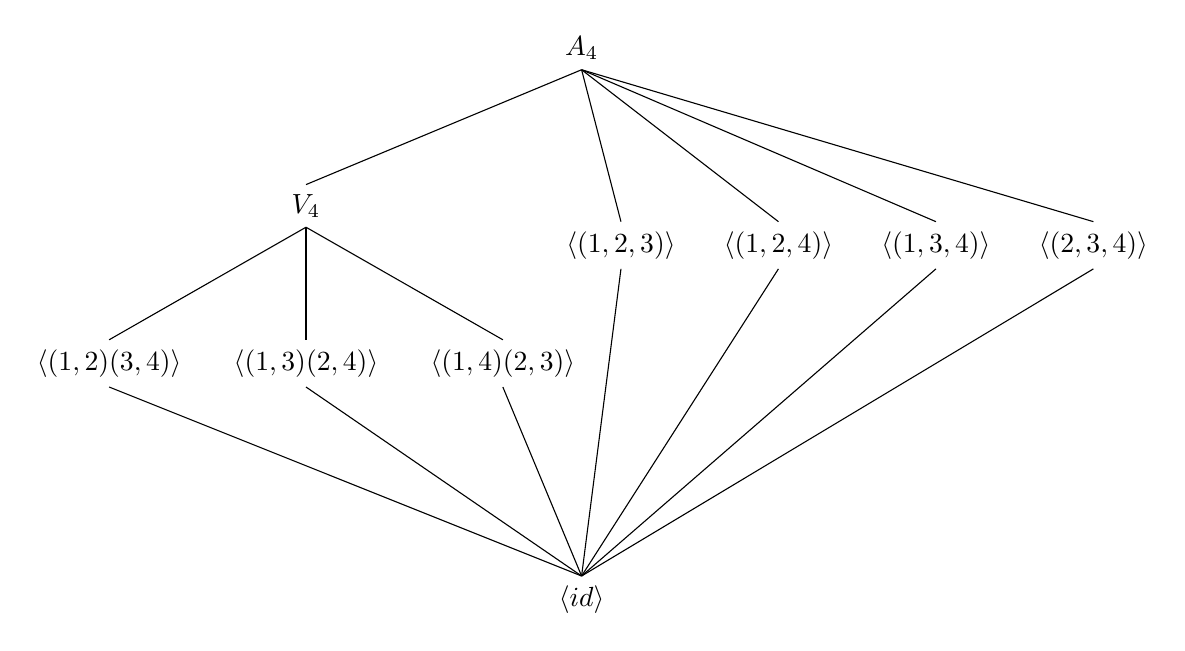
\begin{tikzpicture}
	\node (A4) at (0, 0) {$A_4$};
	\node (V4) at (-3.5, -2) {$V_4$};
	\node (h1) at (-6, -4) {$\span{(1,2)(3,4)}$};
	\node (h2) at (-3.5, -4) {$\span{(1,3)(2,4)}$};
	\node (h3) at (-1, -4) {$\span{(1,4)(2,3)}$};
	\node (h4) at (0.5, -2.5) {$\span{(1,2,3)}$};
	\node (h5) at (2.5, -2.5) {$\span{(1,2,4)}$};
	\node (h6) at (4.5, -2.5) {$\span{(1,3,4)}$};
	\node (h7) at (6.5, -2.5) {$\span{(2,3,4)}$};
	\node (I) at (0, -7) {$\span{id}$};
	\draw[-] (A4.south) -- (V4.north);
	\draw[-] (V4.south) -- (h1.north);
	\draw[-] (V4.south) -- (h2.north);
	\draw[-] (V4.south) -- (h3.north);
	\draw[-] (A4.south) -- (h4.north);
	\draw[-] (A4.south) -- (h5.north);
	\draw[-] (A4.south) -- (h6.north);
	\draw[-] (A4.south) -- (h7.north);
	\draw[-] (h1.south) -- (I.north);
	\draw[-] (h2.south) -- (I.north);
	\draw[-] (h3.south) -- (I.north);
	\draw[-] (h4.south) -- (I.north);
	\draw[-] (h5.south) -- (I.north);
	\draw[-] (h6.south) -- (I.north);
	\draw[-] (h7.south) -- (I.north);
	\end{tikzpicture}
\end{center}
And the subgroup lattice of $A_4/V_4$ looks like this:
\begin{center}
	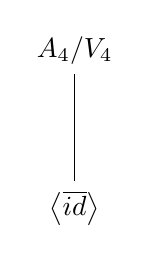
\begin{tikzpicture}
	\node (A4) at (0, 0) {$A_4/V_4$};
	\node (V4) at (0, -2) {$\span{\overline{id}}$};
	\draw[-] (A4.south) -- (V4.north);
	\end{tikzpicture}
\end{center}
Compare the structure of the subgroup lattice above $V_4$ in the subgroup lattice of $A_4$. It has the exact same structure as the subgroup lattice of $A_4/V_4$. So we notice (again) that $\pi$ is an \textbf{order preserving bijection}.

\pagebreak
\subsection{`Additional Relation'}
\prob{4.5.20.} First, deduce that \(\Z[\i]/\) will be isomorphic to \(\Z_{10}\) because \(1+3\i = 0\) gives `\(10 = 0\)'. Now define a ring homomorphism
\[
	\psi = \pi \times \imath_\Z : \Z \ra \Z[\i] \ra \Z[\i]/\ideal{1+3\i}
\]
We will show that \(\ker \psi = 10\Z\). It is enough to show that \(\ker \psi \leq 10\Z\). For any \(a\in \ker\psi\), \(a\) is also an element of \(\ideal{1+3\i}\), thus there exists some \(m+n\i\in \Z[\i]\) such that \(a = (1+3\i)(m+n\i)\). Then we have
\[
	a = (m-3n) + (3m + n)\i\in \Z \implies a = m - 3n, 3m+n = 0
\]
Thus \(a = m - 3n = m - 3(-3m) = 10m \in 10\Z\), therefore \(\ker\psi  = 10\Z\). Next we show that \(\psi\) is surjective. From the relation \(1+3\i = 0\), multiplying \(\i\) on both sides give \(\i = 3\). Then any element \(m+n\i \in \Z[\i]\) can be written as \(m+3n\in \Z\). Thus \(\psi\) is surjective, and by the First Isomorphism Theorem,
\[
	\Z_{10} = \Z/\ker\psi \approx \im\psi = \Z[\i]/\ideal{1+3\i}
\]
(\textbf{Generalization}) If \(\gcd(a, b) = 1\), the following holds.
\[
	\Z[\i]/\ideal{a+b\i} \approx \Z_{a^2+b^2}
\]

\pagebreak~
\end{document}
